\chapter{The Differ and Patcher components}\label{chap:DifferAndPatcher}
Inside the FiGA approach, the application of changes to source code does not occur directly, but it first passes through diagram modification. The diagram that represents the executing application code is modified instead of source code in order to take advantage of diagram abstraction and at the same time to apply precise changes to code. Obviously, extracting differences between original and modified diagram and applying them to code are two inseparable components of the same sub-process of the FiGA approach. This means that they have to be designed to work together, since the comparator component must know what type of modifications it has to look for and the detail level to use to modify the found differences; the patcher component that applies changes must in turn know how to interprete information provided by the differ component. The interaction between the two components must produce a source code that reflects modified diagram characteristics. Such code is then used to apply modifications on the running instance of considered application using the JavAdaptor tool.

It is important to mark that this part of FiGA process does not have to be necessarily executed by two different programs: all the procedures could be executed by one program that internally manages translation between diagram and code changes. Another solution could be to use already existent programs: once found a software that compares UML diagrams and another one that executes a patch on a given code (or file) it should be possible to make them work together creating (or using) a sort of adapter between them.
The solution presented by this work is an hybrid.
The comparator program, Differ, has been created with the sole aim to found code-mappable diagram differences and to write them down on a file, each one with appropriate details to facilitate and guide code change. Instead, since the component for code patching, Patcher, takes advantage of an already existent command, the linux shell program \textit{patch}, can be seen in two different ways: it is actually an independent user-defined component, created to communicate with the Differ component and to perform code alteration but it can be also seen as an adapter which facilitates the use of the \textit{patch} linux shell command.

\begin{figure}[htbp]
   \centering
   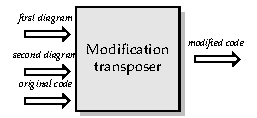
\includegraphics{figs/abstractComp.pdf}
   \hspace{1.5cm}
   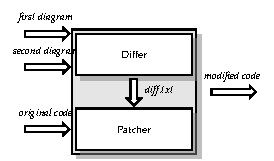
\includegraphics{figs/concreteComp.pdf}
   \vspace*{5pt}
   \caption{Representation of abstract component and current implementations}\label{generic components i/o}
\end{figure}

The two components (independently of their implementations) receive as input the original source code, its UML diagram representation and the modified diagram and return as output the modified source code. Note that the output code has to be patched and annotated so that if it is used to generate its representative diagram, it should be the same (in diagram conception) of modified diagram.
Differ component actually takes as input only original and modified diagrams. It compares them according to Patcher-managed differences and produces a file "diff.txt" which contains the list of all changes to perform on code. It is Patcher component that takes as input the original source code and the "diff.txt" file and modifies the provided code by applying the changes it finds inside input text file.
Figure~\ref{generic components i/o} illustrates generic components process and Differ and Patcher actual behaviour.

The importance of producing a source code that can be used to generate UML diagrams reflects the FiGA approach described in figure~\ref{fig:iterative approach}. In fact it must be considered that the final code which must be obtained, could require more iterations of the sub-process composed by diagram modification and code change. For this reason it is crucial that each iteration produces a consistent code which can be represented by a UML diagram.
If this requirement is provided, it makes also possible to apply further changes at a later time, even after a complete cicle of adaptation process, whenever running application needs to be upgraded.
Note that the implementations of components presented in this work consider only one iteration: all changes applied on diagram are transposed on code one by one but during only one execution. More iterations, if necessary, should be managed by the user, who should alter diagrams and call programs every time he wants to perform one iteration.

Following sections illustrate Differ and Patcher components, which are respectively the implementation of the diagram comparator component and the implementation of code manipulator tool.
It is worth to point out that such implementations are test-supported. In fact, there is, for both of them, an appropriate set of tests which check if the two components correctly perform some simple operations. They help components evolution: in fact, they can be used, during implementations improvement, to verify if programs change their behaviour when the same simple operations are performed.

\section{Differ}
Translation from diagram to code changes needs, first of all, to extract all modifications applied to code representative diagram and then to apply them on code. This process can be split in two steps: in the former we compare diagrams and extract differences; in the latter we adapt the source code. The implementation could be performed by one component that manages the whole process or by two different components which performs respectively the comparation and the code manipulation.
Moreover the two components could be implemented in many ways: they could be components created with the precise aim of working with the FiGA framework or could be already existent components adapted to work together.
Here, it is discussed a possible implementation for the first component.

In case of considering already existent programs, let's mark that comparing two diagrams it is a generic task that can be realized by different components. Some of them are able to both visualize diagrams and compare them even showing history modifications. Even if this feature could be useful to have an overview of all changes applied, it concerns a comparison between diagrams in all their aspects (even graphic ones) and could consider some diagram properties that are not directly mappable into code changes. Furthermore, such type of comparation may suppose to give only a generic view of all performed modifications, omitting other important details that could be fundamental to apply changes to code. An example of such type of comparator could be the one provided by IBM Rational Software Architect. Because of difficulties introduced before, that is extreme lack of precision, redundancy of useless details and confusion of modified elements, this work considers to choose the approach of a completely new comparator program.

The first component of this process should then compare two diagrams and return a list of all changes applied in an appropriate way and format. In general, it takes as input original and modified diagrams and produces something that should be easily interpreted by the program chosen to transfer changes to code.

Differ component is the implementation of the component which aims to extract differences between two given diagrams. In particular, this implementation receives as input the original diagram and its modified counterpart in .emx format and once compared them, as seen in figure~\ref{generic components i/o}, produces a file "diff.txt" which contains a list of found differences, already formatted to be applied on a Java source code. 

Differ first aim is to find all differences between two .emx files. An emx file is structured as a Document Object Model file, i.e. as a tree (or a graph) structure composed by nodes, in which each node symbolizes a diagram element. Figure~\ref{fig:DOMtree} gives a written and graphic representation of used diagram files.
\begin{figure}[htbp]
  \centering
  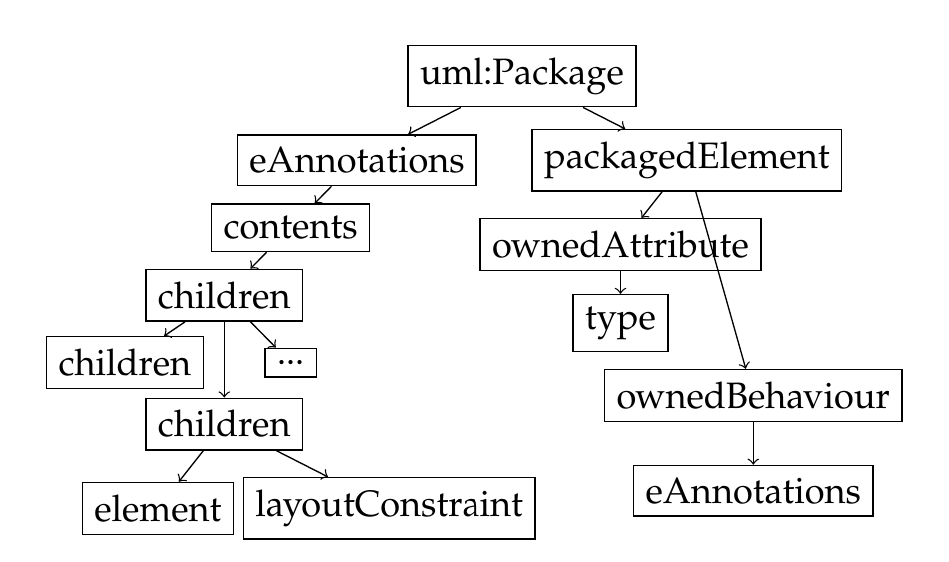
\includegraphics[width=.7\textwidth]{figs/DOMtree}\\
  \showxml{es1.xml}\vspace*{10pt}
\caption{Example of .emx file and relative tree graph}\label{fig:DOMtree}
\end{figure}
Such a tree representation can be easily interpreted also as a graph, since nodes have internal fields which can indicate different types of relationship with other nodes using the ID (a sequence of letter and numbers) which univocally labels each node. For example, inside an activity diagram, an action "actionA" is represented by a DOM node. If such action is followed by an action "actionB", they are linked by an arrow: such arrow is in turn represented by another DOM node but it is not a child or a sibing of action nodes. Their relationship is indicated by internal fields of DOM node. In this case "actionA" has an internal field called \textit{outgoing} which contains the ID of the arrow DOM node. The arrow node has, instead, a \textit{target} field which contains "actionB" ID. In this way a relationship between DOM nodes is established even if they are not apparently connected inside the DOM tree. That is why an emx (or xml) file can also be seen as a graph.
In particular in this work to well-analyse such type of file graph structure can not be ignored since to extract necessary diagram details, nodes relationships are fundamental.

The huge problem that emerges is that comparing two graphs, and in particular recognize their isomorphism,  is known, in algorithm literature, to be a NP problem, i.e. it belongs to the set of decision problems solvable in polynomial time by a theoretical non-deterministic Turing machine. However it is not clear yet if it is a P (problem solvable with a deterministic Turing machine in polynomial time) or NP-complete problem (that is a NP problem which all reduction are NP), because no polynomial time algorithm is known. Graph isomorphism is then still an open problem in NP according to~\cite{Garey} terminology and as~\cite{GraphsIso} explains. 

To overcome such a problem, Differ takes advantage of the extreme specificity of its aim, that is to extract only code-mappable changes and, in particular, ones managed by Patcher component.
Thus, instead of applying a comparation that from all differences filters what is appliable to a source code, that is an approach from higher to lower level, directly does a targeted research, i.e. it looks only for a predefined set of changes.

In order to follow such approach, it takes advantage of a xml format characteristic: each node has its own ID, that is a literal and numeric sequence that univocally identifies it. Relationships between nodes, inside emx file, are expressed by name of relationship and related node ID.

In general, Differ approach is to look for differences in a particular order, so that, when changes are performed on code following given order there are not errors due to elements erroneous changes. For each type of element Differ component usually, at firstm looks for deleted elements, then for modifications of kept ones and, at last, for added elements. For a more precise idea of the necessary modification order that have to be applied on code, and then to be produced by Differ, look at section~\ref{sect:operatorsOrder}.

For each element of the diagram, Differ creates a list of IDs of elements belonging to original diagram and one of elements belonging to modified one.
In order to create such lists, it executes a depth-first search of the tree structure of the emx file, identifying each node type and filtering all types of nodes it is not looking for. When, during the search, it finds a node with requested type, it inserts the node ID inside the list.
After that, it applies set operations to extract sub-lists of deleted elements (IDs belonging only to original diagram), added ones (IDs belonging only to modified diagram) and potentially changed elements (the intersection between the two lists of IDs). It then proceeds browsing each list and adding the respective code change operator to file "diff.txt".

\begin{apitable}[h]{Class diagram add operators}{class add operators}

\apititle{addClass}
\apimember{void addClass(String name, String visibility, boolean isAbstract)}{Creates a new file name.java  and inside it a class declaration with given visibility. If isAbstract is true the declared class is abstract}

\apititle{addInterface}
\apimember{void addInterface(String name, String visibility)}{Creates a new file name.java  and inside it an interface declaration with given visiility}

\apititle{addField}
\apimember{void addField(String name, String visibility, String type, String className, boolean isStatic)}{Opens the file className.java and writes inside it a field declaration with given name, visiility and type. If isStatic is true the declared field is also static}

\apititle{addMethod}
\apimember{void addMethod(String name, String visibility, String returnType, String parametersTypeAndNames, String className, boolean isAbstract, boolean isStatic)}{Opens the file className.java and writes inside it a method declaration with given name, visiility and returnType and parameters with their respective names. If isStatic is true the declared method is also static and if isAbstract is true then the method is declared as abstract}

\apititle{addConstructor}
\apimember{void addConstructor(String visibility, String paramsTypeAndName, String className)} {Opens the file className.java and writes inside it a constructor declaration with the name of the class and with given visiility and parameters with their respective names}

\apititle{addGeneralization}
\apimember{void addGeneralization(String sourceClass, String destClass)} {Opens the file sourceClass.java and adds at the end of class declaration the keyword "extends" and then the name destClass}

\apititle{addImplementation}
\apimember{void addImpl(String sourceClass, String destInterf)} {Opens the file sourceClass.java and adds at the end of class declaration the keyword "implements" and then the name destInterf}

\end{apitable} 

\section{Limitations}
Free and uncontrolled manipulation of UML diagrams could generate differences not treated by Differ component and then propagate the error even to code modification.
Here some of the changes that are not or can not be treated are explained.
First of all, inside UML class diagram it is necessary to consider similarity of methods and constructors. User could have the temptation to change a constructor in method or viceversa. This possibility is not contemplated because of the actual differences that distinguish such types of functions. Treating it would mean to check how user performed mutation and thus check, for  example, the presence of return type, the actual renaming of element and the deletion of keyword constructor. It is instead preferable to omit such possibility of change in order to keep a logical behaviour of program.

At Differ level there are some difficulties in managing constructors, in particular empty ones. In fact, when a class diagram is generated from source code, each class contains the empty constructor even if it is not implemented inside source code. Since the diagram comparator component is here thought to be independent from source code and based only on diagrams, the program can not check if each empty constructor is actually declared inside respective classes. That is why Differ treats such alteration as usual and delegates to problem to Patcher component. Thus, if a user deletes or modify an empty constructor, Differ component appends a \textit{modConstructor} or a \textit{deleteConstructor} inside diff.txt file. If such constructor does not exists and the user deletes it Patcher component raises an exception when tries to find it inside Java class. On the contrary if user modifies empty non-existent constructor and Patcher does not find it inside source code, it does not perform any change: this is because of the possibility that user changes a class name and tries to keep diagram consistency renaming also empty constructor.
But this Patcher behaviour is just in case of constructor renaming. It is allowed to modify arguments and visibility of an empty constructor even if it does not exist: Patcher would first create default empty constructor and then modify it.
Some of possible class diagram improvements, regarding code manipulation management, could be addition of exceptions and package operators.

Activity diagram, since it is a little more complicated, is affected by some more limitations.
One of the most simple is the impossibility of renaming activity elements (actions, decisions or loops). If the user wants to rename and action is forced to delete and then recreate it with a different name and the obtained code should be the wanted one.
The most important case that has to be considered is the possibility that Reverse\reflectbox{R}, since it generates only activity components belonging to executed flow, omits some elements.
If the user creates them inside generated activity diagram, Differ considers them as new elements and appends an add operator to diff.txt file. When Patcher executes it, it creates a duplicate of an existing element, causing errors inside code that are propagated to future generated diagrams. Instead, the user must be conscious of actual code structure not to make mistakes.
The same reasoning could be made for decision branches: if the user adds a branch on a decision that already has such type of branch ("then" or "else"), Differ writes down an \textit{addTest} operator and Patcher tries to add an elready existent branch causing code internal disorder.

The most limited comparation of diagram is the one between UML sequence diagrams. Even if at the beginning of Differ implementation the aim was to manage messages order, then an important diagram inaccuracy has been noticed.
If a loop (for example a "while" loop) contains a annotated message and if it is executed more than one time, the representative sequence diagram is composed by lots of messages: such representation it is not precisely-mappable into code context. That is why the idea of managing messages order, that is to permits the swapping of messages, has been rejected.
In order to permit to Differ and Patcher to create a new sequence diagram, the user sholud keep in mind a convention. The lifeline that sends the first messages must have "0" as name: in this way the two programs understand where to create new annotated sequence inside Java classes.
An important lack of sequence diagram is also multithreading management. If the diagram it is generated by a multithread code, and then there are more concurrent lifelines, Differ can not manage the context yet.

For what concerns Patcher limitations, note that it can be considered as a mere executor of Differ-provided operations. It could be not correct, then, to talk about Patcher limitations, since its limitations are all the operations that it does not implement but that Differ notices. However, since presented implementations are the first versions of both programs, they, for definition, are made to be related one another.
